\begin{figure}[t]
\centering
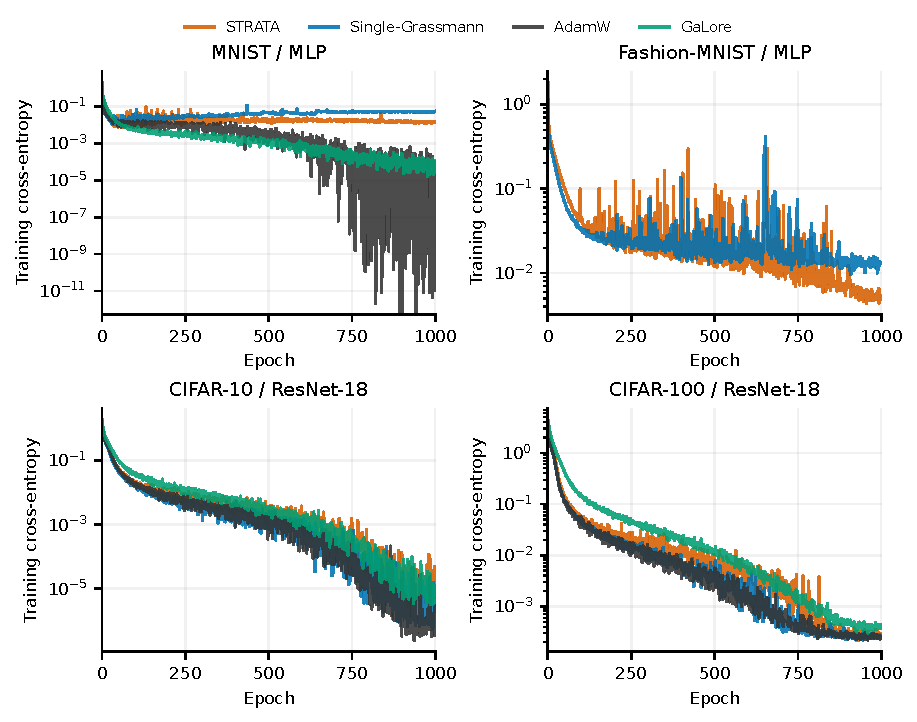
\includegraphics[width=\linewidth]{figures/fig_loss_classification.pdf}
\caption{\textbf{Full 1000-epoch training-loss trajectories.} Four archived classification settings, seed 42. Within each available method grid we select a completed run by terminal-100 validation accuracy and plot its raw training cross-entropy. Baseline grids have unequal sizes; these panels are descriptive convergence comparisons, not an equal-search causal experiment. No smoothing, extrapolation, seed averaging, or test-based selection is used. Training and validation curves for the same runs, every completed classifier-grid loss, fixed-rank PINN curves, graph/continual curves, and separately labeled ongoing runs appear in Appendix~\ref{app:loss-trajectories}.}
\label{fig:loss-classification}
\end{figure}
\paragraph{Loss trajectories and generalization.}
Figure~\ref{fig:loss-classification} replaces endpoint-only inspection with complete recorded optimization paths. Low training cross-entropy does not establish a test-accuracy advantage. The accompanying held-out cross-entropies expose late overfitting and confidence effects that accuracy alone can conceal. Appendix~\ref{app:loss-trajectories} retains both curves and adverse hyperparameter outcomes. All observed epochs are plotted; an archived index of zero is the first logged trained epoch, not a reconstructed common initialization.


\begin{table}[htbp]
\centering
\caption{\textbf{Validation-audited head-to-head endpoints.} PINNs restrict both methods to rank 64 and select by terminal PDE loss. Classifiers select by validation accuracy. Bold compares the two methods; all values use seed 42.}
\label{tab:head-audited}
\begin{adjustbox}{max width=\linewidth}
\begin{tabular}{llrr}
\toprule
Task & Metric & Single-G & STRATA \\
\midrule
burgers & Rel-$L_2$ $\downarrow$ & \textbf{0.02607} & \cellcolor{oursbg}0.02666 \\
burgersg2 & Rel-$L_2$ $\downarrow$ & 0.02617 & \cellcolor{oursbg}\textbf{0.02615} \\
poisson & Rel-$L_2$ $\downarrow$ & 2.04357 & \cellcolor{oursbg}\textbf{0.18741} \\
mnist & Accuracy $\uparrow$ & 0.98011 & \cellcolor{oursbg}\textbf{0.98273} \\
fashion & Accuracy $\uparrow$ & \textbf{0.90328} & \cellcolor{oursbg}0.89907 \\
cifar10 & Accuracy $\uparrow$ & \textbf{0.94034} & \cellcolor{oursbg}0.94014 \\
cifar100 & Accuracy $\uparrow$ & \textbf{0.72574} & \cellcolor{oursbg}0.71402 \\
\bottomrule
\end{tabular}
\end{adjustbox}
\end{table}


\begin{table}[t]
\centering
\caption{Archived benchmark endpoints. Bold marks the better of STRATA and Single-Grassmann only; these are single-seed endpoints, not multi-seed estimates.}
\label{tab:main}
\footnotesize
\begin{adjustbox}{max width=\linewidth}
\begin{tabular}{lrrrrl}
\toprule
Task & AdamW & GaLore & Single-G & STRATA & Verdict \\
\midrule
Burgers rel-$L_2$ $\downarrow$ & 0.0286 & 0.436 & \textbf{0.0261} & \cellcolor{oursbg}0.0267 & tie \\
Burgers-g2 rel-$L_2$ $\downarrow$ & 0.0486 & -- & 0.0262 & \cellcolor{oursbg}\textbf{0.0262} & tie \\
Poisson rel-$L_2$ $\downarrow$ & 0.0079 & -- & 2.0436 & \cellcolor{oursbg}\textbf{0.1874} & SG unstable \\
MNIST acc. $\uparrow$ & 0.987 & 0.985 & 0.9801 & \cellcolor{oursbg}\textbf{0.9827} & tie \\
Fashion acc. $\uparrow$ & -- & -- & \textbf{0.9033} & \cellcolor{oursbg}0.8991 & tie \\
CIFAR-10 acc. $\uparrow$ & 0.9419 & 0.9412 & \textbf{0.9403} & \cellcolor{oursbg}0.9401 & tie \\
CIFAR-100 acc. $\uparrow$ & 0.7358 & 0.7051 & \textbf{0.7257} & \cellcolor{oursbg}0.7140 & SG slight \\
ogbn-arxiv val acc. $\uparrow$ & 0.7351 & 0.7234 & \textbf{0.7349} & \cellcolor{oursbg}0.7337 & tie \\
\bottomrule
\end{tabular}
\end{adjustbox}
\end{table}

\paragraph{Archived comparison.} Table~\ref{tab:main} and Table~\ref{tab:head-audited} support a restrained conclusion. STRATA becomes stable after the numerical fixes, but it is not a universal improvement over Single-Grassmann. In the archived Burgers, Burgers-g2, MNIST, Fashion, CIFAR-10, and ogbn-arxiv comparisons, the practical conclusion is a tie or near-tie. In CIFAR-100, Single-Grassmann is ahead by 0.0117. In Poisson, STRATA is much better than Single-Grassmann in a grid where the latter is unstable, but full AdamW is still substantially better at 0.0079 versus 0.1874.

\begin{table}[htbp]
\centering
\caption{\textbf{Epoch-axis nesting diagnostics.} First/last values and early/late-half means use the complete retained diagnostic trajectory. Spearman $\rho$ uses recorded epochs. Diagnostic trends do not establish a performance ranking.}
\label{tab:dnest}
\begin{adjustbox}{max width=\linewidth}
\begin{tabular}{lrrrrr}
\toprule
Task & First & Last & Early mean & Late mean & $\rho$ \\
\midrule
ogbn-arxiv & 0.047 & 0.493 & 0.330 & 0.477 & +0.998 \\
MNIST & 0.309 & 0.204 & 0.249 & 0.204 & -0.766 \\
Fashion & 0.322 & 0.345 & 0.344 & 0.335 & -0.065 \\
Burgers & 0.880 & 0.690 & 0.416 & 0.618 & +0.901 \\
Poisson & 0.573 & 0.415 & 0.287 & 0.407 & +0.822 \\
CIFAR & 0.512 & 0.601 & 0.397 & 0.434 & +0.224 \\
\bottomrule
\end{tabular}
\end{adjustbox}
\end{table}


\paragraph{$\delta_{\mathrm{nest}}$ is descriptive.} The epoch-axis rejudgment is crucial. Graph is unique only in its low starting point, approximately 0.05, followed by collapse to about 0.49. It is not unique in rising: Burgers and Poisson also rise strongly, with Spearman correlations 0.901 and 0.822, and Burgers after its short initial dip has Spearman 0.993. Because rising, flat, and falling diagnostics all map mostly to head-to-head ties, $\delta_{\mathrm{nest}}$ is useful for describing gradient structure but not for predicting STRATA's performance.

\paragraph{A5 mechanism ablation.} Setting $a_1=\cdots=a_K=a_\perp$ makes $\Gamma^a=0$ in the linear surrogate, while coordinatewise Adam remains basis dependent (Appendix~\ref{app:theory-full}). Equalizing scalar layer weights does not substantially degrade the tested cells: in Burgers at lr $5\times10^{-3}$ and rank 64, full STRATA gives 0.0267 and A5 gives 0.0270; in Poisson at lr $5\times10^{-4}$ and rank 32, full STRATA gives 0.0603 and A5 gives 0.0673. These archived cells alone do not establish a benefit from distinct layer weights. The new PubMed controls below test a different empirical regime, with every intervention and adverse outcome retained.


\paragraph{New complete comparison cohorts.}
Table~\ref{tab:new-cohorts} includes a cohort only when all five methods have completed the stated budget. Two-rate rows require all ten trials before validation-based learning-rate selection; fixed-rate rows use $3\times10^{-4}$ for every method. An incomplete search is not reported as a validation-selected winner.
\begin{table}[t]
\centering\footnotesize
\caption{New full-budget comparison cohorts, seed 42, terminal-100 test accuracy. A two-rate search selects each method using terminal validation accuracy. Fixed-rate rows use no rate selection. Only complete five-method cohorts are shown; the full ledger retains every completed trial.}
\label{tab:new-cohorts}
\setlength{\tabcolsep}{3pt}
\begin{adjustbox}{max width=\linewidth}
\begin{tabular}{llrrrrr}\toprule
Task/model & Protocol & STRATA & Single-G & AdamW & GaLore & Indep.\\\midrule
CiteSeer/gat & 2-rate val & \cellcolor{oursbg}0.5676 & 0.5918 & 0.5737 & \textbf{0.6264} & 0.5718 \\
CiteSeer/gcn & 2-rate val & \cellcolor{oursbg}0.4920 & 0.5156 & 0.5927 & \textbf{0.6166} & 0.5030 \\
CiteSeer/gcnii & 2-rate val & \cellcolor{oursbg}0.4751 & 0.4987 & 0.6085 & \textbf{0.6150} & 0.5042 \\
CiteSeer/sage & 2-rate val & \cellcolor{oursbg}0.5575 & 0.5398 & 0.5530 & \textbf{0.6512} & 0.5584 \\
Cora/gat & 2-rate val & \cellcolor{oursbg}0.6980 & 0.7191 & 0.7100 & \textbf{0.7816} & 0.7365 \\
Cora/gcn & 2-rate val & \cellcolor{oursbg}0.7012 & 0.7164 & 0.7154 & \textbf{0.7718} & 0.6956 \\
Cora/gcnii & 2-rate val & \cellcolor{oursbg}0.6898 & 0.7014 & 0.6784 & \textbf{0.7603} & 0.6934 \\
Cora/sage & 2-rate val & \cellcolor{oursbg}0.4653 & 0.6506 & 0.7060 & \textbf{0.7503} & 0.5641 \\
PubMed/gat & 2-rate val & \cellcolor{oursbg}0.7117 & 0.7431 & 0.7232 & \textbf{0.7663} & 0.7366 \\
PubMed/gcn & 2-rate val & \cellcolor{oursbg}0.7174 & 0.7121 & 0.7045 & \textbf{0.7592} & 0.6878 \\
PubMed/gcnii & 2-rate val & \cellcolor{oursbg}0.6634 & 0.7107 & 0.7088 & \textbf{0.7499} & 0.6693 \\
PubMed/sage & 2-rate val & \cellcolor{oursbg}0.7162 & 0.6790 & 0.6906 & \textbf{0.7580} & 0.7415 \\
adult/MLP-256-256 & 2-rate val & \cellcolor{oursbg}0.8149 & 0.8149 & 0.8172 & \textbf{0.8216} & 0.8117 \\
adult/MLP-512-512 & 2-rate val & \cellcolor{oursbg}0.8151 & 0.8128 & \textbf{0.8191} & 0.8184 & 0.8151 \\
cifar100\_class\_shift/ResNet18-CIFAR & 2-rate val & \cellcolor{oursbg}0.5309 & \textbf{0.5737} & 0.5584 & 0.5306 & 0.5337 \\
cifar10\_label\_shift/ResNet18-CIFAR & 2-rate val & \cellcolor{oursbg}0.7501 & 0.7665 & \textbf{0.8021} & 0.8000 & 0.7696 \\
covertype/MLP-256-256 & 2-rate val & \cellcolor{oursbg}0.9622 & 0.9630 & \textbf{0.9635} & 0.9627 & 0.9615 \\
covertype/MLP-512-512 & 2-rate val & \cellcolor{oursbg}0.9664 & 0.9664 & 0.9645 & 0.9660 & \textbf{0.9675} \\
Rotated-MNIST/MLP (fine-tuning) & 2-rate val & \cellcolor{oursbg}0.5765 & 0.5711 & \textbf{0.6219} & 0.5969 & 0.5728 \\
Rotated-MNIST/MLP (replay) & 2-rate val & \cellcolor{oursbg}0.8858 & 0.8717 & \textbf{0.9072} & 0.8888 & 0.8714 \\
rotated\_mnist\_shift/MLP-256-256 & 2-rate val & \cellcolor{oursbg}0.9761 & 0.9790 & \textbf{0.9806} & 0.9796 & 0.9767 \\
wine\_red/MLP-256-256 & 2-rate val & \cellcolor{oursbg}0.6842 & 0.6883 & 0.7102 & \textbf{0.7185} & 0.6910 \\
wine\_red/MLP-512-512 & 2-rate val & \cellcolor{oursbg}\textbf{0.7150} & 0.6970 & 0.7149 & 0.7105 & 0.7018 \\
wine\_white/MLP-256-256 & 2-rate val & \cellcolor{oursbg}0.7242 & 0.7317 & 0.7204 & 0.7260 & \textbf{0.7389} \\
wine\_white/MLP-512-512 & 2-rate val & \cellcolor{oursbg}0.7088 & 0.7231 & 0.7174 & 0.7100 & \textbf{0.7389} \\
\bottomrule\end{tabular}
\end{adjustbox}\end{table}
After completing both rates on Cora/GCN, validation selects STRATA $3\times10^{-4}$ and Single-Grassmann $10^{-3}$. Their test accuracies are 0.70120 and 0.71643; the earlier positive fixed-rate difference therefore does not survive the completed search. GaLore reaches 0.77180 in this cohort. This adverse comparison is retained.
On the completed PubMed/SAGE two-rate cohort, STRATA reaches 0.71623 versus Single-Grassmann 0.67902, a descriptive gain of 3.721 percentage points. The highest test accuracy among the validation-selected methods is 0.75801 (galore); this single-seed observation does not establish a graph-family advantage.
\paragraph{Completed Rotated-MNIST replay protocol.} Both fine-tuning and replay use the same seed-42 split (55000 training, 5000 validation and 10000 test examples), two 256-wide hidden layers, rank 64, and ten rotations from $0^\circ$ to $90^\circ$ in $10^\circ$ increments. Each rotation receives 100 epochs. Replay stores 200 examples after each task and adds one recalled example per four current-task examples in each minibatch (current batch size 512); all five methods use this same replay rule. Endpoints average epochs 901--1000, evaluating all ten seen rotations. Every method completes both original rates before terminal validation accuracy selects the rate: $10^{-3}$ for STRATA, AdamW, GaLore and Independent, and $3\times10^{-4}$ for Single-Grassmann. STRATA improves on Single-Grassmann by 1.412 percentage points and on Independent by 1.443 points; AdamW and GaLore remain higher. These single-seed comparisons do not establish statistical significance. The loss curves retain all selected methods without smoothing; the mean validation loss covers an increasing set of seen rotations at task boundaries.

